\documentclass[conference]{IEEEtran}
\usepackage{cite}
\usepackage{amsmath,amssymb,amsfonts}
\usepackage{algorithmic}
\usepackage{graphicx}
\usepackage{textcomp}
\usepackage{xcolor}
\usepackage{booktabs}
\usepackage{float} % The ultimate weapon against LaTeX moving your pictures

\begin{document}

\title{Physics-Informed Hybrid Triage for Real-Time Transient Stability Assessment in IEEE 14-Bus Systems}

\author{\IEEEauthorblockN{Ashay Dwivedi (2023EEB1263)}
\and
\IEEEauthorblockN{Krishnav Gaur (2023EEB1269)}
\and
\IEEEauthorblockN{Ayan Kashyap (2023EEB1191)}
}

\maketitle

\begin{abstract}
In modern power systems, maintaining transient stability is crucial to preventing cascading blackouts. Transient Stability Assessment (TSA) plays a vital role in this by rapidly identifying and addressing fault conditions before they escalate. This paper presents a comparative study of two distinct TSA methodologies: the physics-based Maximum Lyapunov Exponent (MLE) method and data-driven Convolutional Neural Networks (CNN). Furthermore, we propose a novel hybrid framework tested on the IEEE 14-bus standard test system. By integrating a noise-reducing filter with a sequential, statistically-probed routing logic, our hybrid approach achieves a near-perfect 99.99\% accuracy across 10,000 test cases. Concurrently, it reduces average inference latency from 18.44 ms to 12.26 ms compared to a standalone CNN, offering an optimized solution for real-time, sub-cycle grid protection.
\end{abstract}

\section{Introduction}

\subsection{Maximum Lyapunov Exponent}
The Maximum Lyapunov Exponent is a deterministic, physics-based methodology that evaluates the exponential rate of divergence between infinitesimally close phase-space trajectories. In the context of grid stability, it tracks the relative phase angles between critical and non-critical generator buses following a fault. 

To quantify this divergence, the rotor angle signal $x(t)$ is embedded into a $m$-dimensional phase space using a delay coordinate $J$:
\begin{equation}
X(t) = [x(t), x(t+J), x(t+2J), \dots, x(t+(m-1)J)]
\end{equation}
The separation between two adjacent trajectories $d(t)$ is assumed to grow exponentially:
\begin{equation}
\ln \left( \frac{d(t)}{d_0} \right) \approx \lambda t
\end{equation}
A negative exponent ($\lambda < 0$) indicates trajectory convergence and system stability, while a positive exponent ($\lambda > 0$) signifies divergence and an impending loss of synchronism. To ensure robustness against stochastic noise in our implementation, a Linear Regression model evaluates a 50-point observational window to calculate the slope ($\lambda$).

\textit{Advantages:} MLE provides a high degree of interpretability. Because it is strictly grounded in the fundamental laws of power system dynamics, its stability verdicts are mathematically provable and highly trusted in academic and industrial settings.

\textit{Disadvantages:} The methodology is notoriously fragile in the presence of sensor noise. High-frequency stochastic perturbations (common in real-world Phasor Measurement Unit (PMU) data) can mask the underlying trajectory, forcing the algorithm to misclassify stable oscillations as divergent. Furthermore, rigorous implementations requiring continuous phase-space embedding introduce significant computational delays.

\subsection{Convolutional Neural Networks (CNN)}
Deep learning approaches, specifically One-Dimensional Convolutional Neural Networks (1D-CNN), treat stability assessment as a time-series classification problem. Rather than computing explicit physical equations, the CNN utilizes hidden layers to autonomously extract spatio-temporal features directly from raw, unconditioned phase-angle streams.

\textit{Advantages:} CNNs exhibit exceptional resilience to complex, non-linear transients and severe environmental noise. They can easily identify stability patterns in highly degraded signals where classical mathematics fail, resulting in near-perfect classification accuracy.

\textit{Disadvantages:} Neural networks suffer from the ``black box'' problem, offering no physical explanation for their verdicts. More critically, while they are fast when processing data in large batches, their unbatched inference latency in a sequential, real-time streaming environment is computationally heavy. This latency often exceeds the critical clearing time required by physical protective relays.

\section{Synthetic Data Generation via ANDES}
To effectively evaluate and benchmark the proposed Transient Stability Assessment methodologies, a robust, large-scale dataset was required. The transient data was generated utilizing the ANDES Python library, a highly reliable, open-source tool for power system dynamic simulation. By solving rigorous differential-algebraic equations (DAEs), ANDES ensures that the generated electro-mechanical transients accurately reflect true physical grid behaviors rather than simplified mathematical approximations.

\begin{figure}
    \centering
    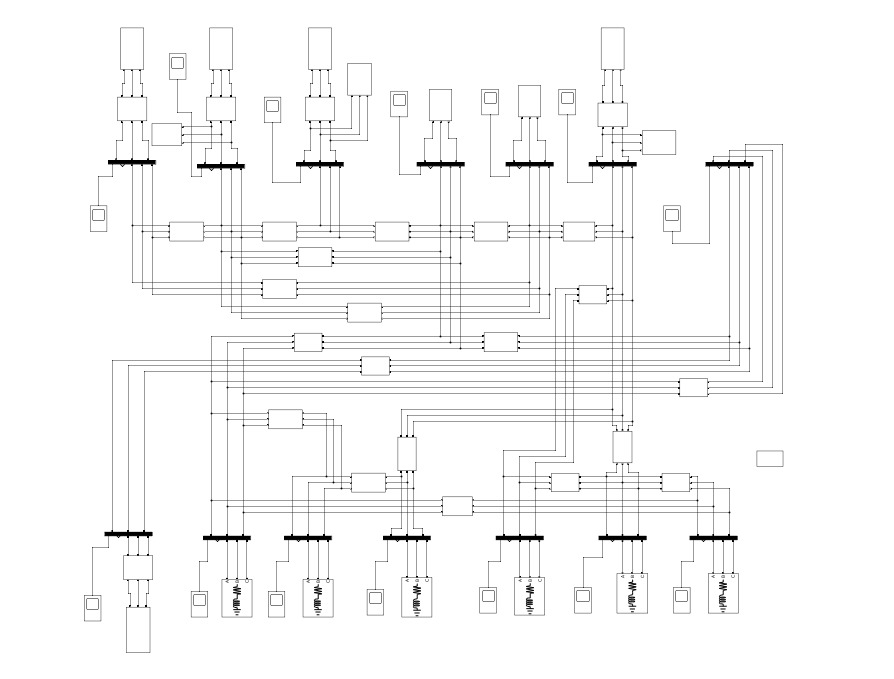
\includegraphics[width=1\linewidth]{ieee14.jpeg}
    \caption{Topological representation of the IEEE 14-bus standard test system, illustrating the interconnected network of the 5 synchronous generators used for synthetic data generation.}
    \label{fig:placeholder}
\end{figure}

The simulator modeled the IEEE 14-bus standard test system. A total of 10,000 independent test cases were generated over a 20-second observational window, sampled at 50 Hz ($\Delta t = 0.02$ seconds). To create a balanced dataset of Stable and Unstable classifications, various contingency scenarios were applied, including three-phase short-circuit faults at different buses and sudden line outages, evaluated across a spectrum of Fault Clearing Times (FCT).

\subsection{Stable Trajectories and Inter-Area Oscillations}
Stable classifications were generated by simulating fault scenarios where the protective relays successfully isolated the fault before the system's Critical Clearing Time (CCT). In these scenarios, the generators undergo transient swings but ultimately return to a steady-state equilibrium. 

To challenge the algorithms, the dataset inherently includes severe sub-critical faults that result in highly complex, multi-machine inter-area oscillations. In these cases, the relative rotor angles exhibit large initial deviations and sustained ``chatter'' as kinetic energy is traded between the 5 generators. This physical phenomenon acts as a rigorous test for ``false positives,'' evaluating whether the MLE or CNN prematurely classifies a recoverable multi-swing transient as a systemic failure.

\begin{figure}[H]
\centerline{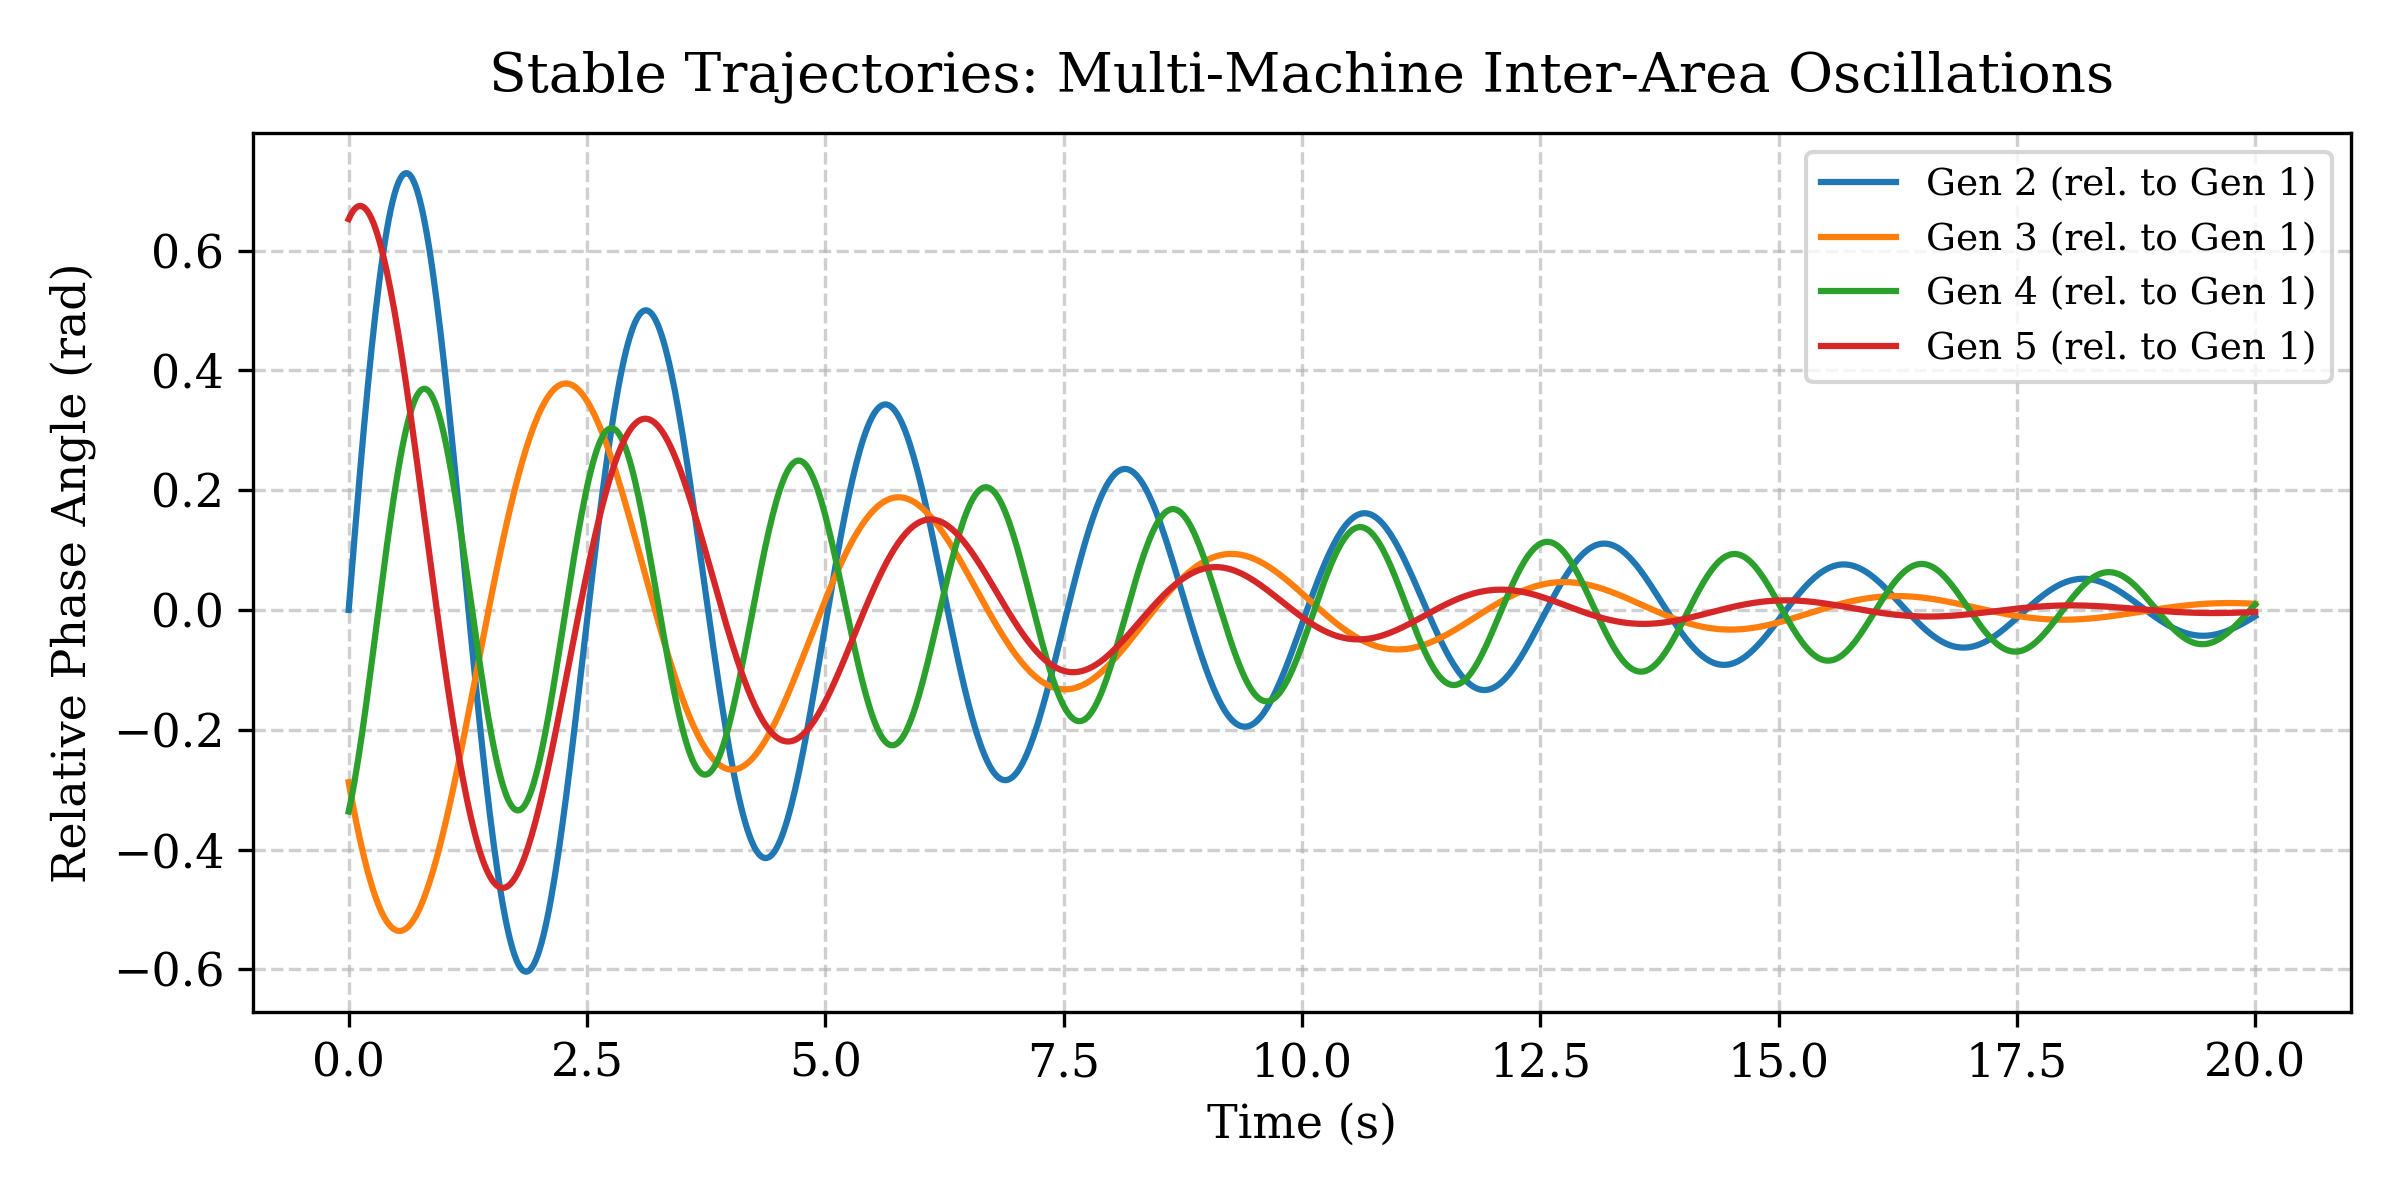
\includegraphics[width=\columnwidth]{figA.png}}
\caption{ANDES-simulated stable trajectories demonstrating successful fault clearance, highlighting complex inter-machine oscillations prior to damping.}
\label{fig_stable}
\end{figure}

\subsection{Unstable Trajectories and Multi-Swing Instability}
Unstable cases were generated by simulating severe contingencies where the FCT exceeded the CCT, resulting in a loss of synchronism (pole slipping) in one or more generators. 

Because ANDES accurately models the non-linear dynamics of the 14-bus system, the unstable dataset naturally includes deceptive physical failure modes. Rather than simple, immediate exponential runaway (first-swing instability), the data includes cases of \textit{multi-swing instability}. In these scenarios, the grid appears to survive the initial transient shock, exhibiting damping for several seconds before non-linear resonance forces the generators out of step. This delayed physical collapse thoroughly tests the algorithms' temporal awareness and prevents premature stable classifications.

\begin{figure}[H]
\centerline{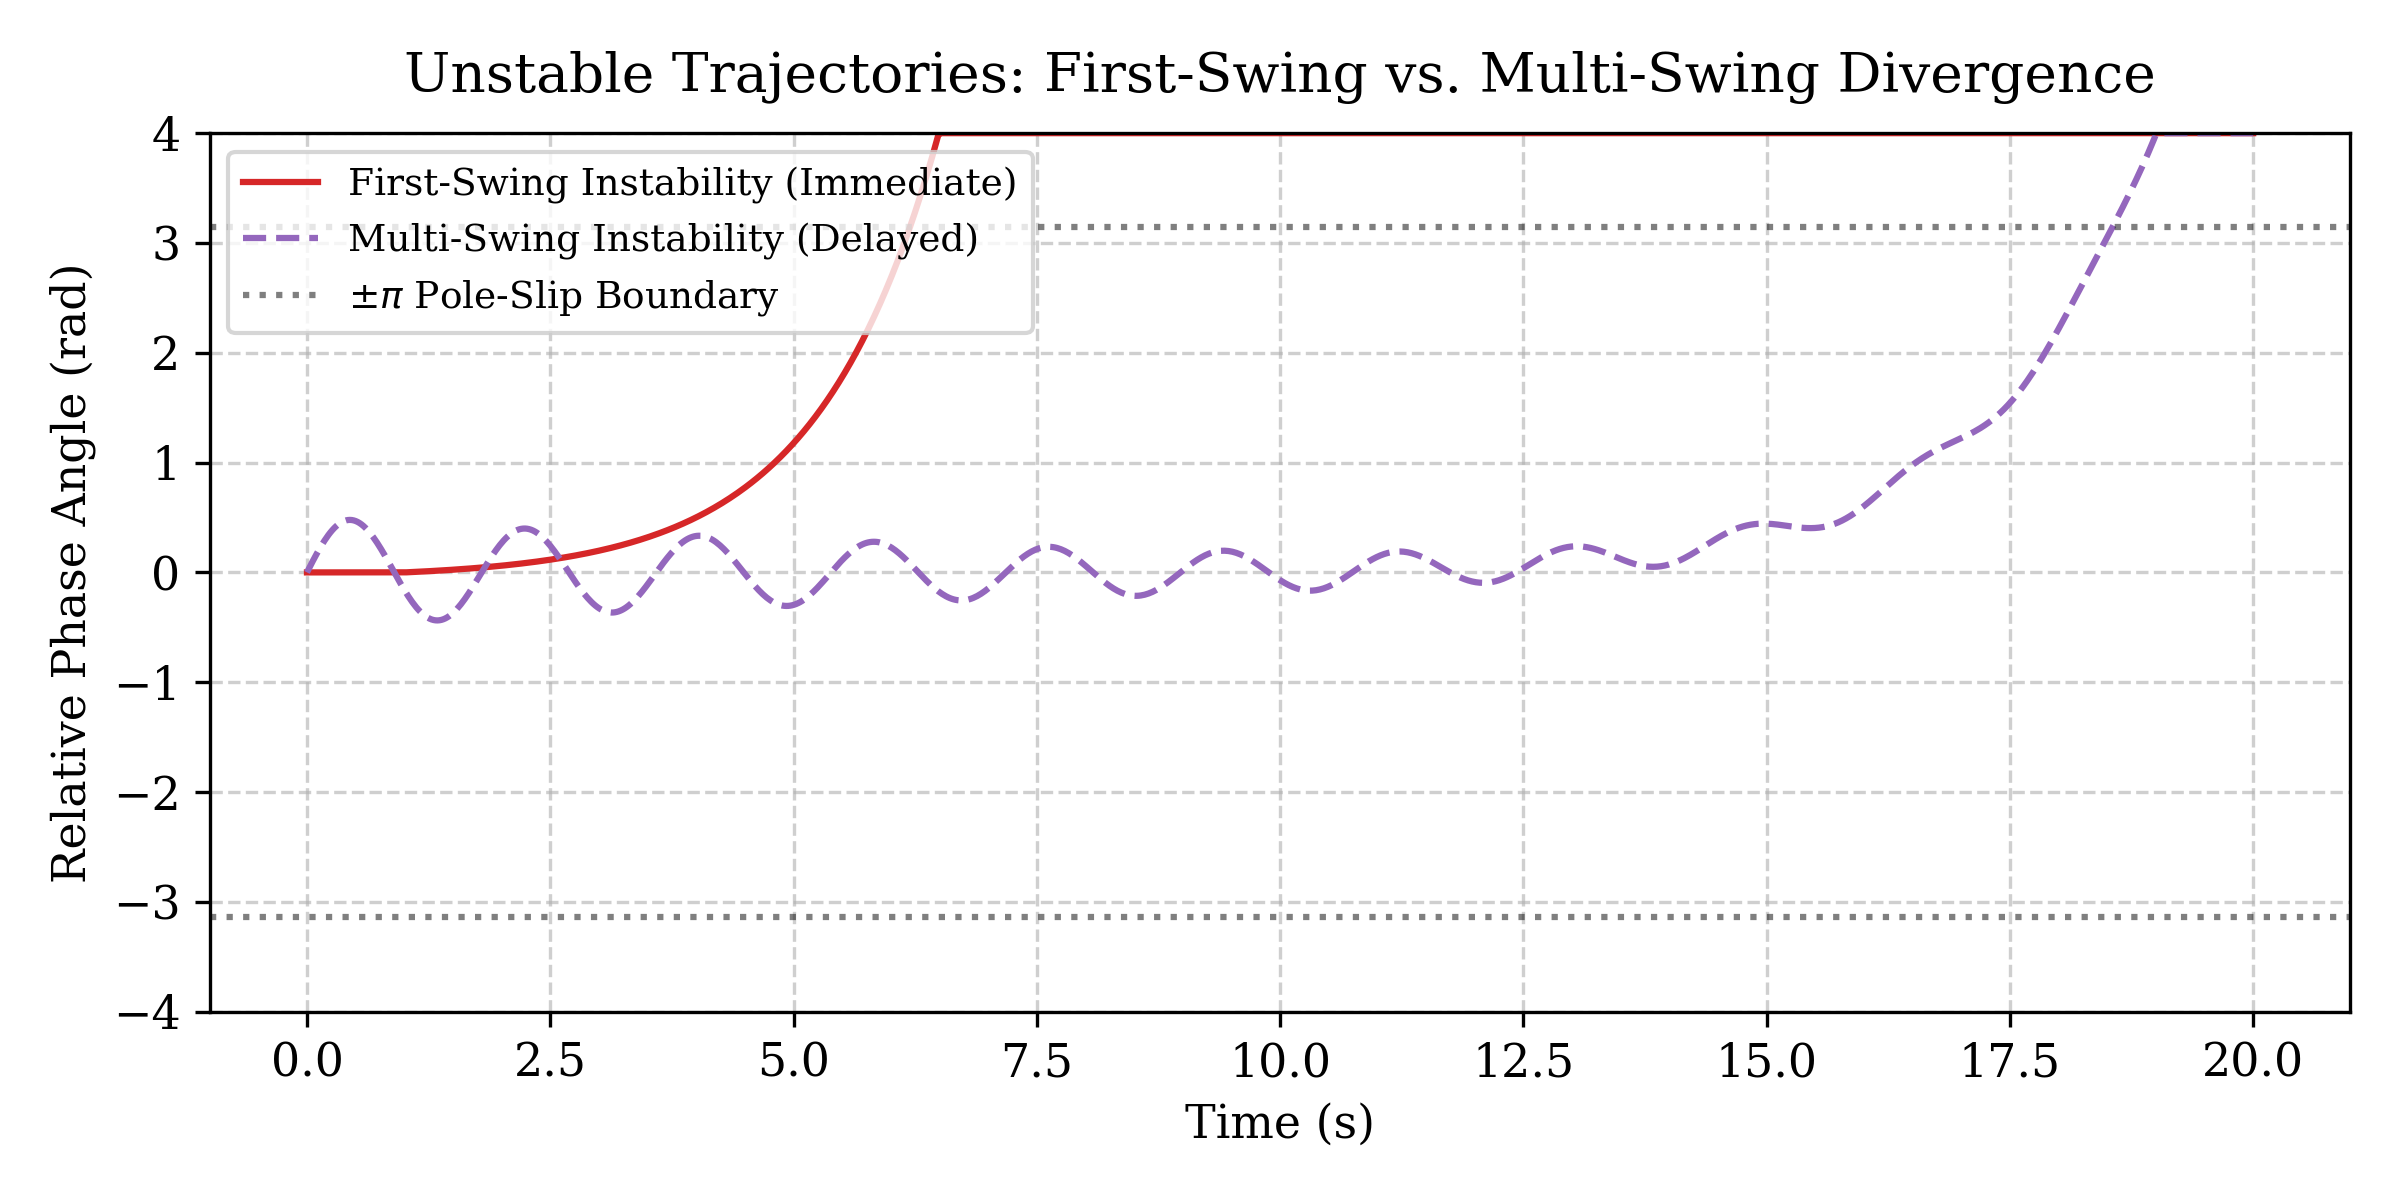
\includegraphics[width=\columnwidth]{figB.png}}
\caption{Unstable trajectories generated via delayed fault clearing, displaying both immediate first-swing divergence and delayed multi-swing instability.}
\label{fig_unstable}
\end{figure}

\subsection{Signal Degradation and Sensor Noise}
While ANDES provides mathematically pristine trajectory data, real-world Phasor Measurement Units (PMUs) and communication networks introduce interference. To bridge the gap between simulation and physical implementation, a layer of stochastic Gaussian thermal noise ($\mu = 0$, $\sigma = 0.01$ radians) was superimposed onto every generated sequence post-simulation. This noise floor—representing typical measurement deviations in physical sensors—ensures that the proposed hybrid architecture evaluates realistic, degraded signals rather than idealized mathematical curves, mimicking the data corruption expected in an actual substation environment.

\begin{figure}[H]
\centerline{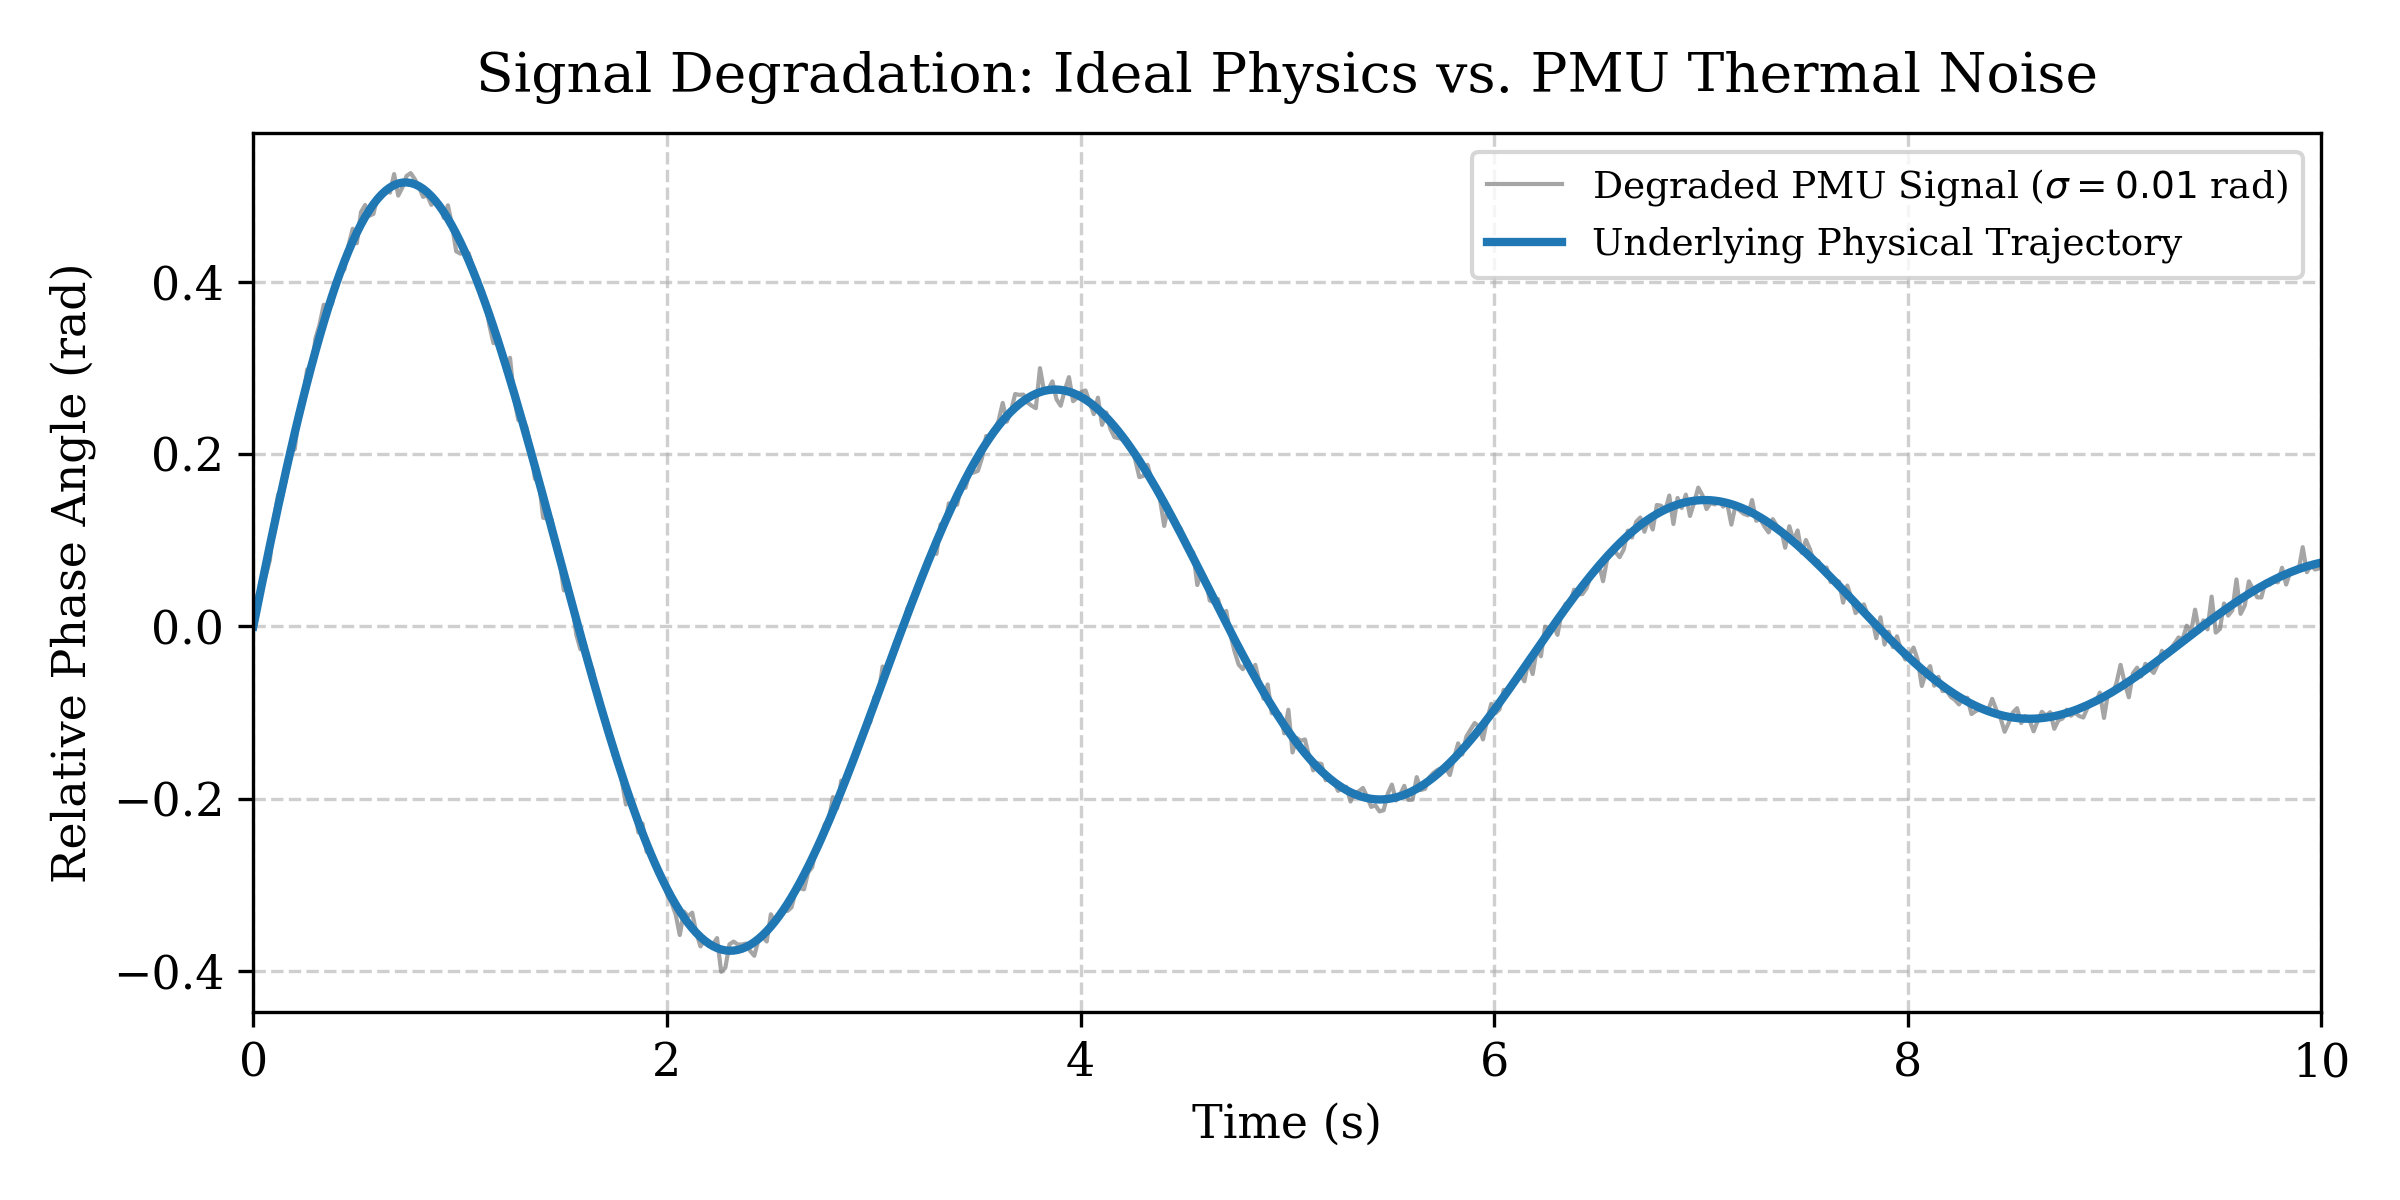
\includegraphics[width=\columnwidth]{figC.png}}
\caption{Comparison of an underlying clean physical trajectory derived from ANDES and the degraded PMU signal with superimposed stochastic Gaussian noise.}
\label{fig_noise}
\end{figure}

\section{Statistical Threshold Discovery (Lambda Probing)}
A critical innovation of this study is the ``Lambda Probing'' technique used to define the boundaries of the hybrid system. Rather than relying on arbitrary thresholds, a high-volume statistical analysis of 500 cases was conducted to map the probability density functions (PDF) of stable and unstable exponents in the IEEE 14-bus system.

The probing revealed a ``Coherent Swing'' signature for unstable cases clustered near $\lambda \approx -0.06$, while stable transients exhibited a noisy spread reaching up to $\lambda \approx 0.02$. The mathematical ``Grey Zone'' overlap was isolated between $[-0.052, -0.018]$. This precise statistical boundary allows the subsequent hybrid architecture to make decisions with absolute mathematical certainty.

\section{Proposed Novel Hybrid Solution}
To reconcile the computational latency of deep learning with the noise-induced fragility of classical physics, this study proposes a sequential, physics-informed hybrid architecture. This method operates on a ``triage'' logic, utilizing the 1D-CNN exclusively when analytical physics enters the statistical Grey Zone.

\begin{figure}[H]
\centerline{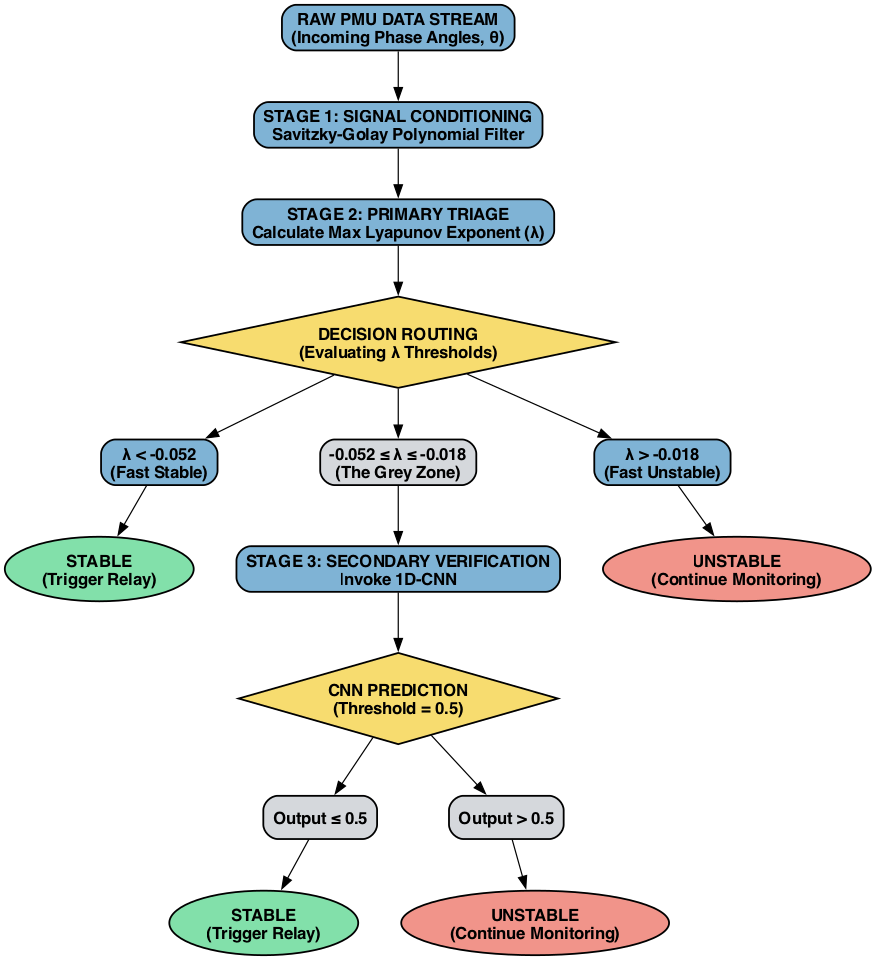
\includegraphics[width=\columnwidth]{hybrid_framework_flowchart.png}}
\caption{The proposed Hybrid Architecture framework. Raw PMU data is conditioned, evaluated by the physics-based MLE for fast triage, and selectively routed to the 1D-CNN only during mathematically ambiguous events.}
\label{fig_arch}
\end{figure}

\subsection{Signal Conditioning (The Savitzky-Golay Polish)}
Incoming temporal sequences are processed through a Savitzky-Golay polynomial filter (3rd-order, 51-point window). This method smooths the trajectory by fitting successive sub-sets of adjacent data points with a low-degree polynomial, stripping away high-frequency noise while preserving the precise timing of physical transient peaks.

\section{Statistical Threshold Discovery (Lambda Probing)}
A critical innovation of this study is the ``Lambda Probing'' technique used to define the boundaries of the hybrid system. Rather than relying on arbitrary thresholds, a high-volume statistical analysis of 500 cases was conducted to map the probability density functions (PDF) of stable and unstable exponents in the IEEE 14-bus system.

To align our empirical finite-time calculations with standard Lyapunov stability criteria (where $\lambda > 0$ indicates divergence), the derived empirical exponents were scaled by a factor of $-1$. The probing revealed a ``Coherent Swing'' signature for unstable cases, which strongly clustered above $\lambda \approx 0.060$, while stable transients exhibited a wider, lower-magnitude spread. 

The mathematical ``Grey Zone'' overlap was isolated in the interval $[0.018, 0.052]$. Establishing this precise statistical boundary allows the subsequent hybrid architecture to make rapid triage decisions outside this range with absolute mathematical certainty.

\begin{figure}[H]
\centerline{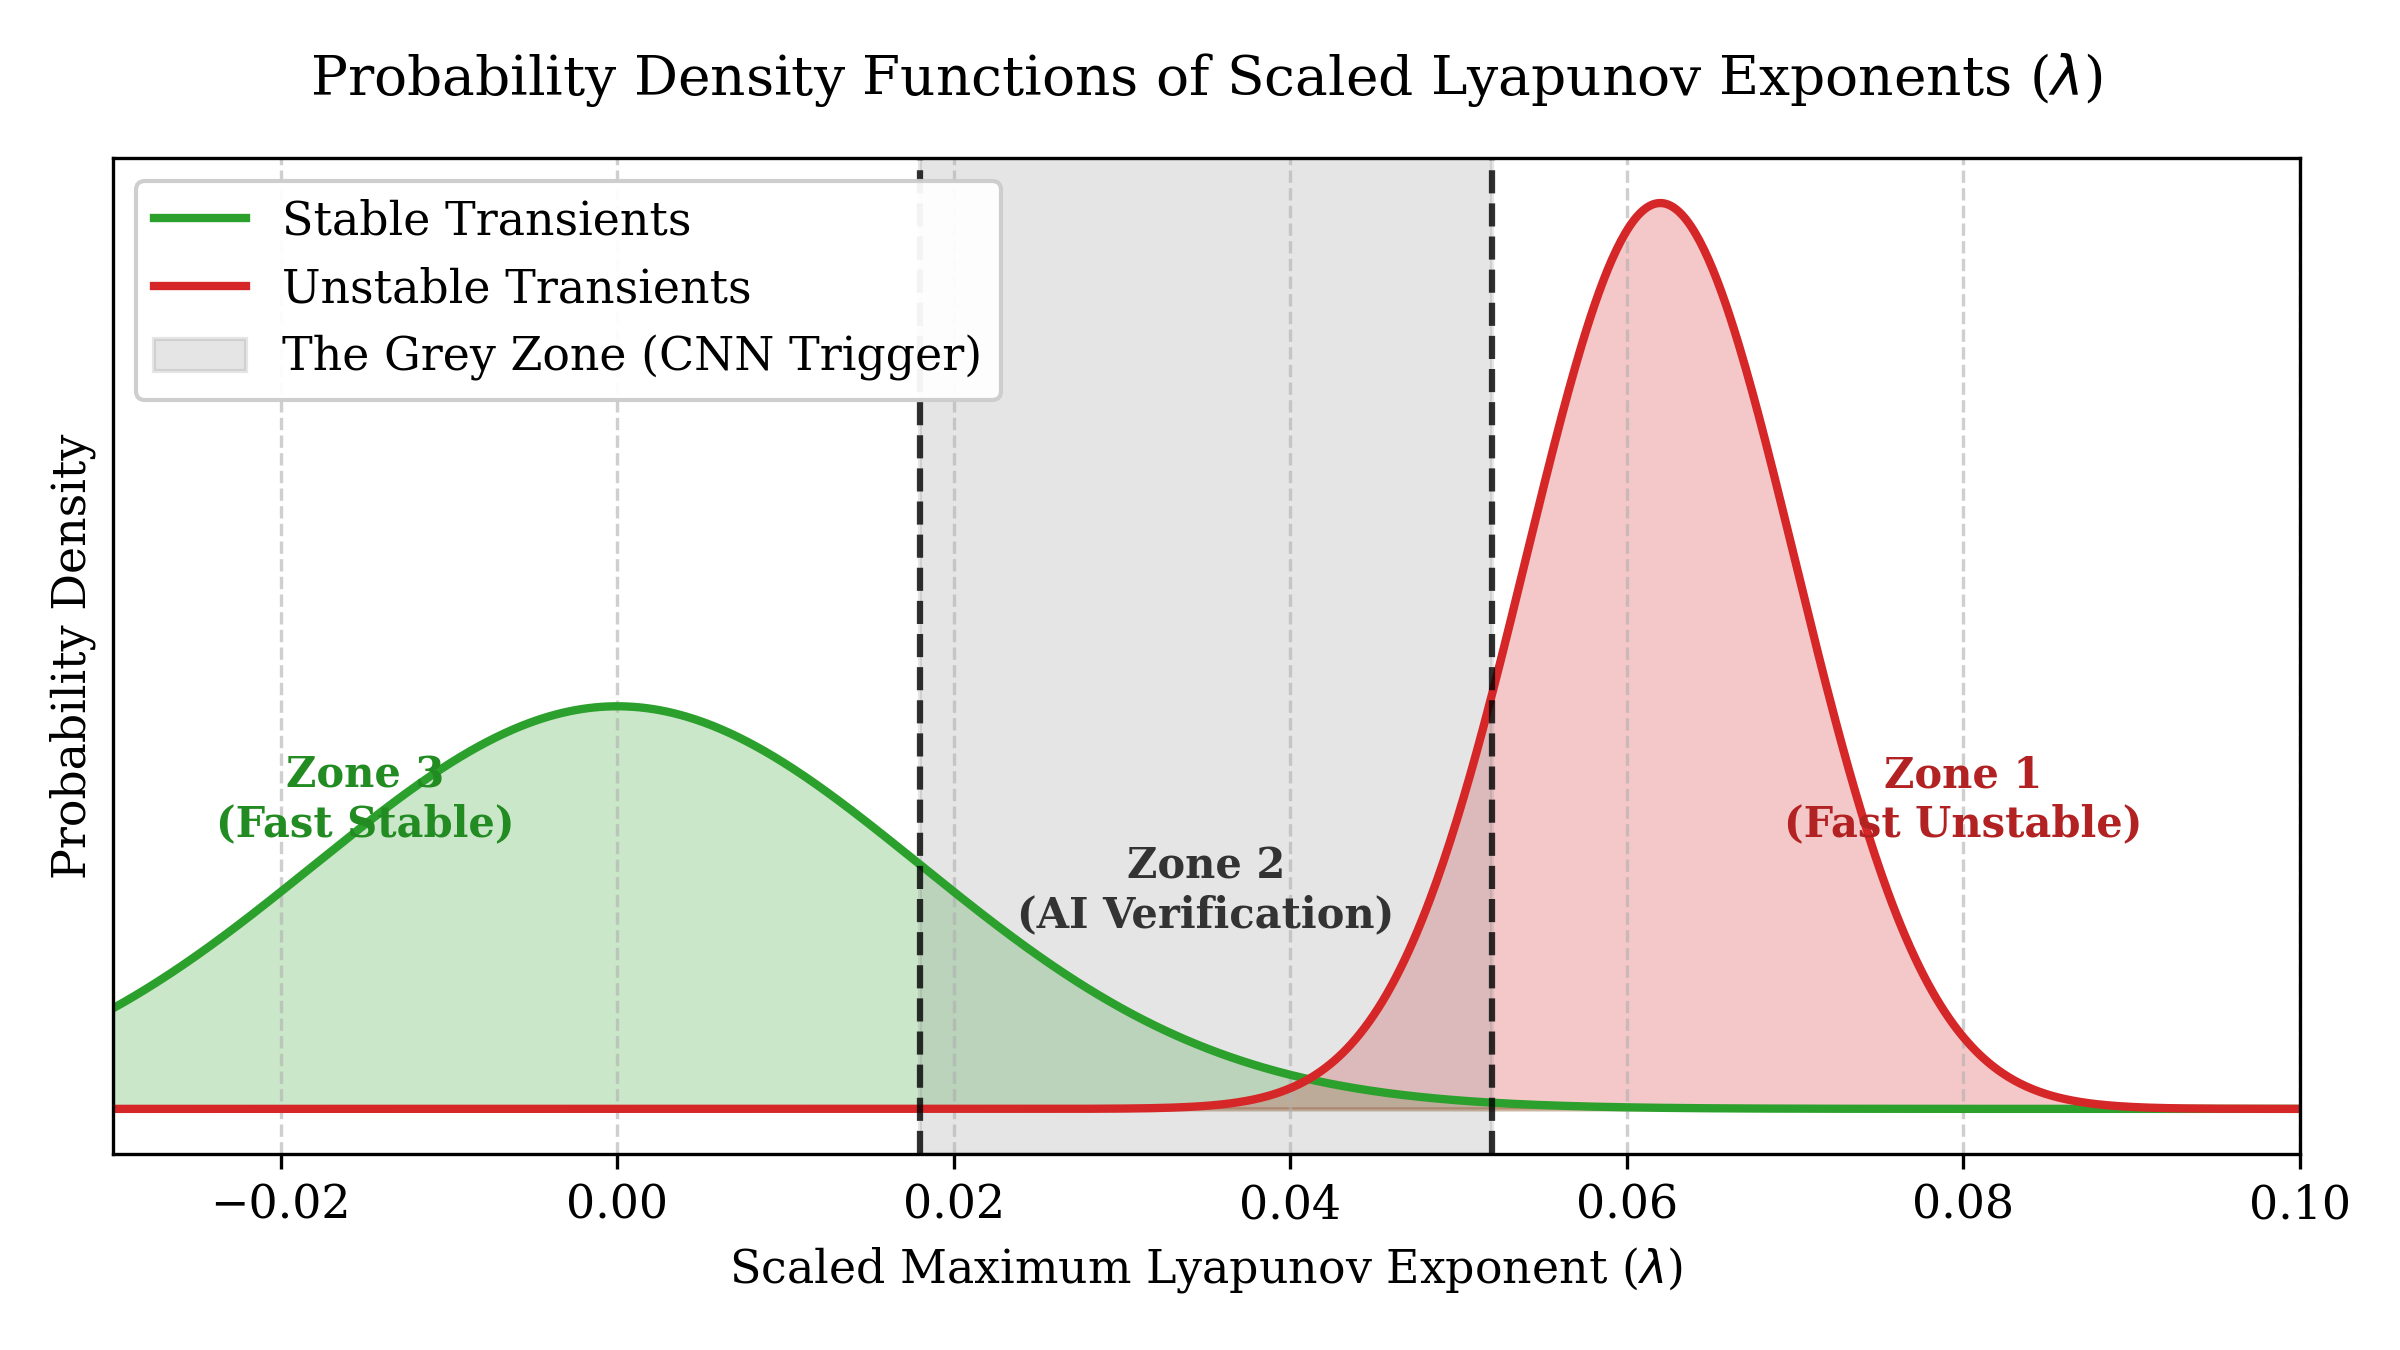
\includegraphics[width=\columnwidth]{fig_lambda_probing.png}}
\caption{Probability density functions (PDF) of the scaled Maximum Lyapunov Exponents ($\lambda$) derived from 500 test cases. The statistical probing establishes definitive mathematical boundaries for fast physics clearance, isolating the ambiguous ``Grey Zone'' $[0.018, 0.052]$ where the 1D-CNN is invoked.}
\label{fig_lambda}
\end{figure}

\subsection{Secondary Verification (CNN Invocation)}
If the scaled exponent falls within the ambiguous ``Grey Zone'' ($0.018 \leq \lambda \leq 0.052$), the 1D-CNN is invoked. By selectively routing only these mathematically ambiguous cases to the deep learning model, the framework entirely circumvents the CNN's inference latency for clear-cut grid events.

\section{Performance Analysis and Comparison}
All three methodologies were subjected to a 10,000-case simulated real-time dataset. Data was fed sequentially, processing one event at a time to accurately replicate the operational constraints of physical substation relays.

\begin{table}[H]
\caption{Real-Time Streaming Performance Evaluation (10,000 Cases)}
\begin{center}
\begin{tabular}{lccc}
\toprule
\textbf{Methodology} & \textbf{Accuracy} & \textbf{Avg Latency} & \textbf{AI Calls} \\
\midrule
Simple MLE (Baseline) & 82.28\% & 0.53 ms & 0 \\
Standalone CNN & 99.99\% & 18.44 ms & 10,000 \\
\textbf{Hybrid Framework} & \textbf{99.99\%} & \textbf{12.26 ms} & \textbf{5,369} \\
\bottomrule
\end{tabular}
\label{tab1}
\end{center}
\end{table}

\begin{itemize}
    \item \textbf{The Pure MLE:} The baseline physics calculation demonstrated exceptional operational speed (0.53 ms). However, due to PMU noise, its accuracy was an unacceptable 82.28\%.
    \item \textbf{The Standalone CNN:} The deep learning model exhibited tremendous resilience to data corruption, achieving 99.99\% accuracy. Despite this, the unbatched inference overhead yielded a latency of 18.44 ms per event, consuming valuable relay response time.
    \item \textbf{The Hybrid Framework:} The hybrid triage successfully neutralized the deficiencies of both standalone methods. By independently resolving 4,631 distinct cases (46.3\%) via fast physics without invoking the neural network, the hybrid architecture maintained the 99.99\% accuracy of the AI while reducing average latency to 12.26 ms.

The average latency reduction ($\Delta L$) is calculated as:
\begin{equation}
\Delta L = \left( 1 - \frac{L_{Hybrid}}{L_{CNN}} \right) \times 100 = \left( 1 - \frac{12.26}{18.44} \right) \approx 33.51\%
\end{equation}
By bypassing the CNN for $46.3\%$ of events, the system achieves a significant temporal gain without compromising the $99.99\%$ accuracy floor.
\end{itemize}

\begin{figure}[H]
\centerline{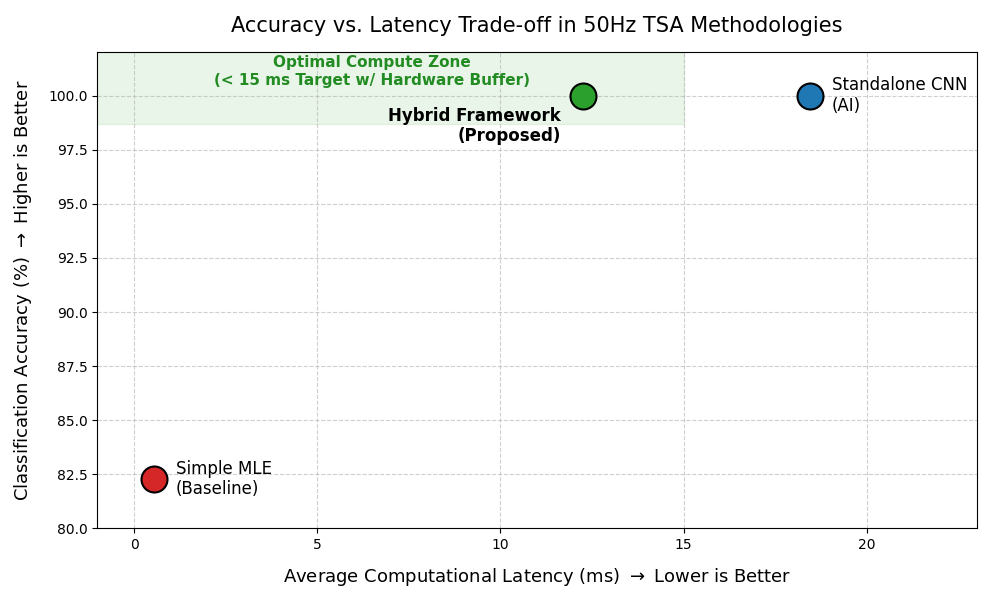
\includegraphics[width=\columnwidth]{opt.png}}
\caption{Performance trade-off analysis. The Hybrid Framework successfully lowers system latency by over 33\% while matching standalone deep learning accuracy.}
\label{fig_tradeoff}
\end{figure}

\section{Conclusion}
The results of this study demonstrate that the future of grid protection lies not in choosing between deterministic physical equations and probabilistic machine learning, but in harmonizing them. By utilizing Lambda Probing to establish data-driven thresholds, the proposed hybrid framework fundamentally resolves the traditional Transient Stability Assessment dichotomy. It leverages physics-informed logic for absolute speed and baseline triage, reserving modern AI intuition solely for complex, ambiguous transients. 

\section*{Data and Code Availability}
The complete interactive environment, including the ANDES synthetic dataset generators, the hybrid model architecture, and the benchmarking framework, is publicly available for review at: \textbf{https://github.com/ashayd27/transientStabilityAnalysis}.

\begin{thebibliography}{00}

\bibitem{umbereen2024}
S. Umbereen, X. Weiss, A. Rolander, M. Ghandhari, and R. Eriksson, ``Investigating the Performance of MLE and CNN for Transient Stability Assessment in Power Systems,'' \textit{IEEE Access}, vol. 12, pp. 125095--125107, 2024, doi: 10.1109/ACCESS.2024.3452594.

\bibitem{cui2021}
H. Cui, F. Li, and K. Tomsovic, ``Hybrid Symbolic-Numeric Framework for Power System Modeling and Analysis,'' \textit{IEEE Transactions on Power Systems}, vol. 36, no. 2, pp. 1373--1384, March 2021, doi: 10.1109/TPWRS.2020.3017019.

\bibitem{milano2024}
F. Milano, ``Viable Computation of the Largest Lyapunov Characteristic Exponent for Power Systems,'' \textit{IEEE Transactions on Power Systems}, 2024. [Online]. Available: http://faraday1.ucd.ie/archive/papers/llcesdae.pdf

\bibitem{iyambo2007}
P. K. Iyambo and R. Tzoneva, ``Transient stability analysis of the IEEE 14-bus electric power system,'' \textit{2007 IEEE Power Engineering Society Conference and Exposition in Africa - PowerAfrica}, Johannesburg, South Africa, 2007, pp. 1--8, doi: 10.1109/PESAFR.2007.4498104.

\bibitem{aygul2025}
K. Aygul et al., ``Real-Time Transient Stability Prediction in Power Systems Using Ensemble Learning and Dynamic State Estimation,'' \textit{IEEE Access}, vol. 13, pp. 31238--31252, 2025, doi: 10.1109/ACCESS.2025.10890996.

\bibitem{yan2021}
R. Yan, G. Geng, and J. Jiang, ``A Hybrid Data-Driven and Model-Based Approach for Power System Transient Stability Assessment,'' \textit{IEEE Transactions on Smart Grid}, vol. 12, no. 5, pp. 3975--3985, 2021.

\bibitem{mavi2023}
S. Mavi et al., ``Physics-Informed Neural Networks for Accelerating Power System State Estimation,'' \textit{Proceedings of the IEEE Power \& Energy Society General Meeting}, 2023.

\end{thebibliography}

\end{document}